% ===========================
% Columbia MSBA Assignment Template
% Author: Alexandre Sepúlveda de Dietrich
% ===========================
\documentclass[11pt]{article}

% --- Page & typography ---
\usepackage[margin=1in]{geometry}
\usepackage{microtype}
\usepackage{setspace}
\setstretch{1.08}

% --- Math, tables, figures ---
\usepackage{amsmath,amssymb}
\usepackage{siunitx}
\usepackage{booktabs, makecell}
\usepackage{graphicx}
\usepackage{caption}
\usepackage{subcaption}
\usepackage{float}
\usepackage{tikz}
\usetikzlibrary{arrows.meta}

% scale: 1 ft = 0.55 cm
\newcommand{\ftscale}{0.55}
\newcommand{\boardheight}{0.45}


% --- Links & smart refs ---
\usepackage{hyperref}
\hypersetup{
  colorlinks=true,
  linkcolor=blue!55!black,
  urlcolor=blue!55!black,
  citecolor=blue!55!black,
  pdfauthor={Alexandre Sepúlveda de Dietrich},
  pdftitle={MSBA Assignment}
}
\usepackage[nameinlink,capitalize]{cleveref}

% --- Header / footer ---
\usepackage{fancyhdr}

% --- Code listings (Python default); keep English identifiers/comments ---
\usepackage{listings}
\usepackage{xcolor}
\usepackage{inconsolata}

\usepackage[table]{xcolor}
\usepackage{multirow}

% ==========================================================================
% ==========================================================================
% ---------------------------
% CONFIG MACROS (edit per assignment)
% ---------------------------
\newcommand{\coursecode}{IEOR E4004}
\newcommand{\coursetitle}{Optimization Models and Methods}
\newcommand{\assignmenttitle}{Project I --- Childcare Desert Reduction in New York City}
\newcommand{\term}{Spring~2026}
\newcommand{\instructor}{Prof.\ Dr. Yaren Bilge Kaya}
\newcommand{\studentname}{Group 8}
\newcommand{\uni}{aes2399}
\newcommand{\studentemail}{aes2399@columbia.edu}
\newcommand{\dueday}{March 2026}
\newcommand{\logoimg}{ieor.png}

% Toggle: show table of contents (0/1)
\newif\ifshowtoc
\showtoctrue
% Toggle: include Academic Integrity & AI Use section (0/1)
\newif\ifshowai
\showaitrue
% ==========================================================================
% ==========================================================================

% ---------------------------
% Styles & utilities
% ---------------------------
% siunitx numbers & alignment


% Regression helpers
\renewcommand{\arraystretch}{1.15}
\newcommand{\coef}[2]{#1\\ \scriptsize{(#2)}}
\newcommand{\ci}[2]{\shortstack[r]{[\,#1;\,#2\,]}}

% Math shortcuts
\newcommand{\E}{\mathbb{E}}
\newcommand{\Var}{\mathrm{Var}}
\newcommand{\Cov}{\mathrm{Cov}}
\newcommand{\1}{\mathbb{I}}

% LP formatting helpers
\newcommand{\lp}[3]{% #1 = max/min, #2 = objective, #3 = constraints (one per line with \\)
\[
\begin{array}{ll}
\text{#1} & #2 \\
\text{s.t.} & \begin{aligned}
#3
\end{aligned}
\end{array}
\]
}

% Optional: same but boxed (nice for examples)
\newcommand{\lpexpr}[3]{%
\begin{resultbox}
\lp{#1}{#2}{#3}
\end{resultbox}
}


% Graphics default path
\graphicspath{{figures/}}

% Listings: Python style
\definecolor{codebg}{HTML}{F8F8F8}
\definecolor{codeframe}{HTML}{E1E4E8}
\definecolor{codekw}{HTML}{005CC5}
\definecolor{codestr}{HTML}{22863A}
\definecolor{codecom}{HTML}{6A737D}
\definecolor{codegray}{HTML}{6E6E6E}
\lstdefinestyle{pycode}{
  language=Python,
  basicstyle=\linespread{0.98}\ttfamily\footnotesize,
  keywordstyle=\color{codekw}\bfseries,
  stringstyle=\color{codestr},
  commentstyle=\color{codecom}\itshape,
  numbers=left,
  numberstyle=\tiny\color{codegray},
  numbersep=8pt,
  frame=single,
  rulecolor=\color{codeframe},
  framerule=0.3pt,
  backgroundcolor=\color{codebg},
  showstringspaces=false,
  upquote=true,
  tabsize=2,
  keepspaces=true,
  columns=fullflexible,
  breaklines=true,
  breakatwhitespace=true,
  postbreak=\mbox{\textcolor{codegray}{$\hookrightarrow$}\space},
  xleftmargin=1.6em,
  framexleftmargin=1.6em,
  aboveskip=0.8\baselineskip,
  belowskip=0.8\baselineskip,
}
\lstset{style=pycode}

% Header/footer styles
\fancypagestyle{coverstyle}{%
  \fancyhf{}
  \lhead{Columbia University}
  \chead{\coursecode}
  \rhead{\studentname}
  \cfoot{\thepage}
  \renewcommand{\headrulewidth}{0.5pt}
  \renewcommand{\footrulewidth}{0.5pt}
}
\pagestyle{fancy}
\fancyhf{}
\lhead{\coursecode}
\rhead{\assignmenttitle}
\cfoot{\thepage}
\setlength{\headheight}{14pt}
\renewcommand{\headrulewidth}{0.5pt}
\renewcommand{\footrulewidth}{0.5pt}

% A lightweight "Problem" environment scaffold
\newenvironment{problem}[2][] % usage: \begin{problem}[Short name]{Problem N — Title}
{\section{#2 \ifx\relax#1\relax\else\ (\textit{#1})\fi}}
{\vspace{0.6em}}

% A small boxed “Result” callout
\usepackage{mdframed}
\newmdenv[
  linewidth=0.5pt,
  roundcorner=4pt,
  backgroundcolor=black!2,
  skipabove=\baselineskip,
  skipbelow=\baselineskip,
  innertopmargin=6pt,
  innerbottommargin=6pt,
  innerleftmargin=9pt,
  innerrightmargin=9pt
]{resultbox}

% ===========================
\begin{document}
% ===========================

% --- Title page ---
\begin{titlepage}
  \thispagestyle{coverstyle}
  \centering
  \vspace*{0.2cm}
  \if\relax\detokenize{\logoimg}\relax\else
    \includegraphics[width=0.38\textwidth]{\logoimg}
  \fi

  \vspace{0.5cm}
  {\Large \textsc{\coursecode{} — \coursetitle{}} \par}
  \vspace{0.2cm}
  {\LARGE \textbf{\assignmenttitle} \par}
  \vspace{0.3cm}
  {\large \term \par}
  \vspace{0.6cm}
  \noindent\makebox[\linewidth]{\rule{\linewidth}{1.2pt}}

    \vspace{0.9cm}
    \begin{minipage}{0.48\textwidth}
      \raggedright
      \textit{Team}\\
      Alexandre Sep\'ulveda de Dietrich (aes2399)\\
      Rong Ji (rj2754)\\
      Suyi Li (sl5867)\\
      Zichen He (zh2709)\\
      Zipeng Liu (zl3627)
    \end{minipage}\hfill
    \begin{minipage}{0.48\textwidth}
      \raggedleft
      \textit{Instructor}\\
      \instructor\\[4pt]
      \textit{Due}\\
      \dueday
    \end{minipage}

  \vfill
  {\large Department of Industrial Engineering and Operations Research\\Columbia University}
\end{titlepage}

\setcounter{page}{2}

\ifshowtoc
\tableofcontents
\newpage
\fi

% --- Academic Integrity & AI use disclosure ---
\ifshowai
\section*{Academic integrity \& AI use}
AI tools were used only as a writing and formatting assistant. The modeling approach, data preparation, optimization logic, interpretation of results, and final submitted content were produced, reviewed, and validated by the project team. AI assistance was limited to presentation tasks such as \LaTeX{} polishing, wording refinement, and formatting.
\addcontentsline{toc}{section}{Academic integrity \& AI use}
\fi

% --- Executive summary (optional but recommended for longer cases) ---
% \section*{Executive summary}
% In 6–10 sentences, state the problem, data, approach, principal quantitative results (use \num{} or math mode), limitations, and the final recommendation.
% Example numbers in math mode: $R^2=\num{0.613}$, expected margin $\approx \num{44.9}$ dollars.

% ===========================
% PROBLEM BLOCKS (duplicate as needed)
% ===========================
% ===========================
% PROJECT BODY
% ===========================

\section*{Project overview}
\addcontentsline{toc}{section}{Project overview}


\paragraph{Objective.}
This project studies how New York City can reduce childcare deserts at minimum cost by combining expansions of existing childcare facilities with the opening of new facilities. A zipcode is considered underserved when available childcare capacity is too low relative to the local child population. The policy challenge is therefore not only to increase total capacity, but also to ensure that enough capacity is available for children under age \(5\), while accounting for the financial and operational costs of intervention.

\paragraph{Project structure.}
We solve the problem in two stages. In \textbf{Part 1}, we formulate an ideal benchmark model in which the city can expand existing facilities and build new facilities freely within zipcodes. In \textbf{Part 2}, we extend this benchmark to a more realistic planning model by imposing stricter expansion limits, piecewise expansion costs, candidate-site restrictions, and minimum-distance requirements between facilities. This two-step structure is useful because it separates the core allocation logic from the implementation frictions that arise in practice.

\paragraph{Approach.}
The analysis combines data preparation, parameter estimation, and optimization. We first construct zipcode-level demand targets and baseline capacity measures from the provided demographic and childcare datasets. Part 1 then solves an ideal mixed-integer model using those estimated parameters. Part 2 does not build on the Part 1 solution itself; instead, it branches from the same cleaned facility data and the zipcode-level demand table, then adds candidate locations, distance-based screening, and realistic expansion parameters before solving its own mixed-integer model. This distinction matters because the realistic model reuses the shared preprocessing and demand construction, not the intervention decisions from the ideal solve.

\paragraph{Code availability.}
The working code is organized as a seven-stage notebook pipeline in the submitted repository. The workflow first cleans the shared inputs, then estimates and solves the ideal model, then estimates and solves the realistic model, and finally exports the comparison figures used in the report. The notebook pipeline is stored under \texttt{notebooks/}, while the report source is stored under \texttt{report/}. \Cref{fig:code-pipeline-main} summarizes the execution flow.

\begin{figure}[H]
\centering
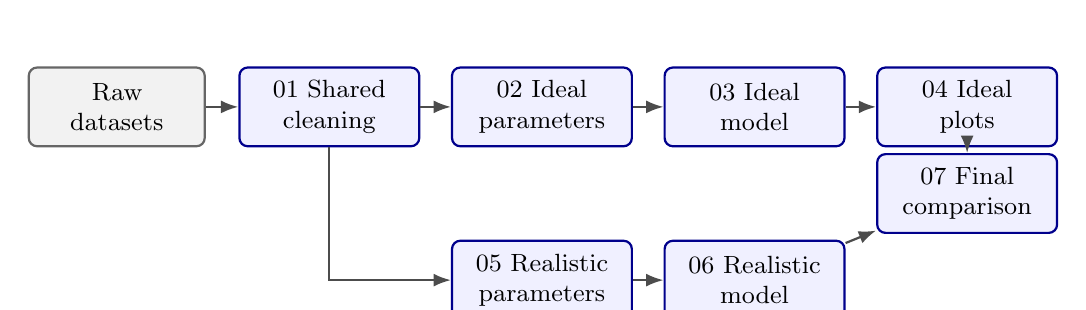
\begin{tikzpicture}[
  font=\small,
  stage/.style={
    draw=blue!55!black,
    thick,
    rounded corners=3pt,
    fill=blue!6,
    align=center,
    minimum height=1.0cm,
    text width=2.05cm
  },
  source/.style={
    draw=black!60,
    thick,
    rounded corners=3pt,
    fill=black!5,
    align=center,
    minimum height=1.0cm,
    text width=2.0cm
  },
  flow/.style={-{Latex[length=2.2mm]}, thick, draw=black!70}
]
  \node[source] (raw) at (0,0) {Raw\\datasets};
  \node[stage] (s1) at (2.7,0) {01 Shared\\cleaning};
  \node[stage] (s2) at (5.4,0) {02 Ideal\\parameters};
  \node[stage] (s3) at (8.1,0) {03 Ideal\\model};
  \node[stage] (s4) at (10.8,0) {04 Ideal\\plots};
  \node[stage] (s5) at (5.4,-2.2) {05 Realistic\\parameters};
  \node[stage] (s6) at (8.1,-2.2) {06 Realistic\\model};
  \node[stage] (s7) at (10.8,-1.1) {07 Final\\comparison};

  \draw[flow] (raw) -- (s1);
  \draw[flow] (s1) -- (s2);
  \draw[flow] (s2) -- (s3);
  \draw[flow] (s3) -- (s4);
  \draw[flow] (s1) |- (s5);
  \draw[flow] (s5) -- (s6);
  \draw[flow] (s4) -- (s7);
  \draw[flow] (s6) -- (s7);
\end{tikzpicture}
\caption{Notebook pipeline used to construct shared inputs, solve both models, and export report figures.}
\label{fig:code-pipeline-main}
\end{figure}

\paragraph{Managerial interpretation.}
From a policy perspective, the problem is a trade-off between two distinct levers. Expanding existing facilities is often cheaper because infrastructure is already in place, but expansion opportunities are limited. New construction is more expensive, but it may be necessary in zipcodes with large shortages or limited existing supply. The optimization model identifies the least-cost mix of these two interventions while meeting both total-capacity and under-\(5\) service requirements.

\section{Part 1: Ideal childcare expansion model}

\subsection{Problem statement}

In the first part of the project, we consider an idealized version of the childcare planning problem. The city is allowed to expand existing facilities and open new childcare centers in any zipcode, without explicit spatial siting restrictions. The objective is to eliminate all childcare deserts at minimum total cost.

A zipcode must satisfy two service requirements in order to be considered adequately covered. First, it must have enough \emph{total childcare capacity}. Second, it must have enough \emph{under-\(5\) childcare capacity}. The total-capacity requirement depends on local socioeconomic conditions. Following the project statement, a zipcode is treated as \emph{high demand} if either its employment rate is at least \(60\%\) or its average income is at most \(\$60{,}000\). In such zipcodes, total capacity must exceed one half of the child population. In all other zipcodes, total capacity must exceed one third of the child population. In every zipcode, under-\(5\) capacity must exceed two thirds of the local population aged \(0\) to \(5\).

This first model deliberately abstracts away from implementation frictions such as land availability and minimum-distance rules. Its purpose is to establish a benchmark: if the city could intervene in the most flexible way possible, what is the least-cost plan required to eliminate all childcare deserts?

\subsection{Data and parameter construction}

\subsubsection{Data cleaning}

Our analysis combines five raw datasets provided for the project. Before estimating model inputs, we first built a consistent data-cleaning pipeline to ensure that all datasets could be merged and used reliably.

We began by standardizing the structure of each file. Unnamed index columns were removed, zipcodes were reformatted into a uniform five-digit string, and variable names were harmonized across datasets. We also converted all relevant quantitative fields, such as capacities, population counts, employment rates, incomes, and coordinates, into numeric format so that later calculations would be based on consistent data types.

Next, we examined missing values and data quality issues. The main missingness appeared in the childcare facility dataset, where some facilities lacked latitude and longitude information. Rather than dropping these records, we retained them and created a flag to indicate missing geographic data, since coordinates are not essential for the ideal model but may matter in the realistic model. After merging the zipcode-level tables, missing employment and income values were imputed with citywide medians, while missing population entries were filled with zero so that the full zipcode universe remained in the planning dataset. We also created basic quality-control flags, including indicators for inactive facilities, zero total capacity, and any inconsistency between \texttt{children\_capacity} and total capacity.

To prepare the supply-side data, we filtered the childcare dataset to active facilities with positive capacity and used \texttt{children\_capacity} as a proxy for current under-\(5\) capacity in the cleaned facility data. On the demand side, we aggregated the population data to create zipcode-level measures of the child population aged \(0\) to \(12\) and the population aged \(0\) to \(5\), and cleaned the employment and income files into zipcode-level lookup tables. The potential locations dataset was also cleaned and assigned unique candidate IDs.

Finally, we constructed a master zipcode table by taking the union of zipcodes from all datasets. This ensured that the merged planning dataset covered the full set of relevant zipcodes rather than only the overlapping subset appearing in every source. As a result, the cleaned data provided a consistent foundation for parameter estimation and optimization.

\subsubsection{Demand-side parameters}

After cleaning the data, we translated the project requirements into model-ready demand parameters.

At the zipcode level, a zipcode \(z\) was classified as high demand if its employment rate was at least \(60\%\) or its average income was at most \(\$60{,}000\). Based on this rule, the required total childcare capacity was defined as one half of the child population aged \(0\) to \(12\) in high-demand zipcodes and one third otherwise. The required under-\(5\) capacity was defined as two thirds of the population aged \(0\) to \(5\). To implement these rules in the optimization model, we converted them into integer requirements:
\[
\mathrm{req\_total}_z =
\begin{cases}
\left\lfloor \dfrac{1}{2}\,\mathrm{pop\_0\_12}_z \right\rfloor + 1, & \text{if zipcode } z \text{ is high demand}\\[1.2ex]
\left\lfloor \dfrac{1}{3}\,\mathrm{pop\_0\_12}_z \right\rfloor + 1, & \text{otherwise}
\end{cases}
\]
and
\[
\mathrm{req\_under5}_z = \left\lceil \dfrac{2}{3}\,\mathrm{pop\_0\_5}_z \right\rceil
\]

This formulation reflects the project definition that a zipcode remains a desert if capacity is less than or equal to the threshold, so the requirement must be strictly exceeded.

For descriptive purposes, we also measured unmet need using
\[
\begin{aligned}
\mathrm{gap\_total}_z &= \max\!\left(0,\ \mathrm{req\_total}_z - \mathrm{existing\_total}_z\right),\\
\mathrm{gap\_under5}_z &= \max\!\left(0,\ \mathrm{req\_under5}_z - \mathrm{existing\_under5}_z\right)
\end{aligned}
\]

These two gap measures summarize the magnitude of the shortage in each zipcode and are used as diagnostic quantities in the analysis, even though the optimization model itself is written directly in terms of required and existing capacity.

\subsubsection{Supply-side parameters}

Existing supply was estimated by aggregating facility-level capacity within each zipcode. Existing total capacity was computed from current licensed capacity, and existing under-\(5\) capacity was approximated using \texttt{children\_capacity}. These aggregated quantities define the baseline level of service already available before any intervention.

At the facility level, for each active facility \(f\), we recorded current total capacity \(n_f\) and under-\(5\) proxy capacity. These values determine both the current supply and the feasible expansion opportunities of existing facilities.

\subsubsection{Expansion cost parameters}

The project statement allows expansion up to \(120\%\) of current capacity, subject to a maximum of \(500\) added slots. After instructor clarification, either
\[
x_f \le \min(1.2\,n_f,\ 500-n_f)
\]
or
\[
x_f \le \min(1.2\,n_f,\ 500)
\]
was acceptable. We adopted the second option in the benchmark notebook, so that
\[
x_f \le \min(1.2\,n_f,\ 500),
\]
where \(x_f\) denotes the number of added slots and
\[
U_f = \min(1.2\,n_f,\ 500)
\]
is the facility-specific upper bound.

The project statement specifies that the first-block per-slot expansion cost \(c_{\text{slots}}(n_f)\) should decrease with current facility size, but it does not provide a closed-form expression. We therefore approximated the first expansion block with size-based per-slot cost tiers for expansions below \(100\%\) of current capacity:
\[
c_f^{(1)} =
\begin{cases}
350, & \text{if } n_f < 25\\
300, & \text{if } 25 \le n_f < 75\\
250, & \text{if } n_f \ge 75
\end{cases}
\]

This specification operationalizes the assignment's statement that the per-slot expansion cost \(c_{\text{slots}}(n_f)\) is decreasing in current facility size while keeping the implementation transparent.

For expansions beyond \(100\%\) of current capacity, we applied the prorated project formula
\[
c_f^{(2)} = \frac{20000 + 200\,n_f}{n_f}
\]

In the corrected benchmark implementation, the optimization model uses a single total expansion variable \(x_f\) together with a binary threshold indicator. If \(x_f < n_f\), the entire expansion is priced at the lower coefficient \(c_f^{(1)}\); if \(x_f \ge n_f\), the entire expansion is priced at the higher coefficient \(c_f^{(2)}\). This matches the assignment's piecewise logic more closely than the earlier additive two-block approximation while remaining MILP-compatible through standard big-\(M\) linking constraints.

\subsubsection{New-facility parameters}

We included the three new-facility options specified in the project: small, medium, and large. Their characteristics are respectively \((100,50,\$65{,}000)\), \((200,100,\$95{,}000)\), and \((400,200,\$115{,}000)\), where each tuple denotes total capacity, under-\(5\) capacity, and fixed construction cost. We also incorporated the additional equipment cost of \(\$100\) for every newly created under-\(5\) slot. Together, these estimated parameters provide the direct inputs for the ideal optimization model. 

\subsection{Optimization model}

\subsubsection{Modeling assumptions}

To keep the benchmark model transparent, we adopt the following assumptions:

\begin{enumerate}
    \item Existing facilities may be expanded up to the maximum allowed by the assignment, subject to the facility-level cap on added slots.
    \item New facilities may be opened in any zipcode.
    \item New facilities come from a discrete menu of sizes, each with a fixed construction cost and a known contribution to total and under-\(5\) capacity.
    \item Demand is enforced at the zipcode level. The model does not represent cross-zipcode commuting or household travel behavior.
    \item Expansion and construction costs follow the project rules, with the unspecified first-block function \(c_{\text{slots}}(n_f)\) approximated by a decreasing three-tier schedule.
    \item The variable \texttt{children\_capacity} is used as a proxy for current under-\(5\) capacity at existing facilities.
    \item A binary threshold indicator is used so that once expansion reaches the current facility size, the entire expansion is priced with the higher prorated coefficient from the project statement.
    \item Under-\(5\) capacity created through expansion and new construction is assigned explicitly through decision variables rather than assumed to follow mechanically from total capacity.
    \item Newly built facilities are not allowed to be expanded within the same planning horizon. 
\end{enumerate}

These assumptions make Part 1 a benchmark planning model rather than a fully operational deployment model. This is intentional: the goal is to first understand the core resource-allocation problem before introducing spatial and implementation constraints in Part 2.

\subsubsection{Decision variables}

Using the cleaned data and estimated parameters, we formulated an integer linear optimization model to determine the minimum funding needed to eliminate childcare deserts across New York City under the project's idealized assumptions.

\noindent
For each existing facility \(f\), we define:
\begin{itemize}
    \item \(x_f\): total added slots at facility \(f\);
    \item \(u_f\): number of under-\(5\) slots assigned within the total expansion at facility \(f\).
    \item \(\delta_f\): a binary variable equal to \(1\) if \(x_f \ge n_f\), so the facility enters the higher-cost expansion regime.
    \item \(w_f\): an auxiliary variable representing the modeled expansion cost at facility \(f\).
\end{itemize}

\noindent
For each zipcode \(z\) and facility size \(s \in S=\{\text{small},\text{medium},\text{large}\}\), we define:
\begin{itemize}
    \item \(y_{zs}\): number of new facilities of size \(s\) built in zipcode \(z\);
    \item \(g_{zs}\): number of under-\(5\) slots assigned within those new facilities.
\end{itemize}

\noindent
All decision variables are restricted to be nonnegative integers.

\subsubsection{Objective function}

The objective is to minimize total funding, which includes three components:
\begin{enumerate}
    \item expansion costs at existing facilities;
    \item fixed construction costs for new facilities;
    \item additional equipment costs of \(\$100\) for each newly created under-\(5\) slot.
\end{enumerate}

\noindent
The objective can be written as
\[
\min \quad
\sum_{f \in F} w_f
+
\sum_{z \in Z} \sum_{s \in S} K_s y_{zs}
+
100\left(\sum_{f \in F} u_f + \sum_{z \in Z} \sum_{s \in S} g_{zs}\right)
\]

\subsubsection{Constraints}

The model includes six main groups of constraints.

First, each existing facility can expand only within its allowable limits:
\[
x_f \le U_f
\qquad \forall f \in F
\]

Second, the number of under-\(5\) slots added through expansion cannot exceed total added slots at the same facility, and the binary threshold variable identifies whether the facility remains below its current size or crosses into the higher-cost regime:
\[
u_f \le x_f,\qquad
x_f \le (n_f-1) + U_f \delta_f,\qquad
x_f \ge n_f \delta_f
\qquad \forall f \in F
\]

Third, big-\(M\) linking constraints force the expansion-cost variable to follow the appropriate regime:
\[
w_f =
\begin{cases}
c_f^{(1)}x_f, & \text{if } \delta_f = 0\\
c_f^{(2)}x_f, & \text{if } \delta_f = 1
\end{cases}
\qquad \forall f \in F
\]

Fourth, each zipcode must satisfy the required total capacity after accounting for existing supply, expansions, and new construction:
\[
\mathrm{existing\_total}_z
+
\sum_{f \in F(z)} x_f
+
\sum_{s \in S} B_s y_{zs}
\ge
\mathrm{req\_total}_z
\qquad \forall z \in Z,
\]
where \(B_s\) is the total capacity of a new facility of size \(s\), and \(F(z)\) is the set of existing facilities located in zipcode \(z\).

Fifth, each zipcode must also satisfy the required under-\(5\) capacity:
\[
\mathrm{existing\_under5}_z
+
\sum_{f \in F(z)} u_f
+
\sum_{s \in S} g_{zs}
\ge
\mathrm{req\_under5}_z
\qquad \forall z \in Z
\]

Finally, under-\(5\) assignments in newly built facilities cannot exceed the under-\(5\) capacity allowed by each facility type:
\[
g_{zs} \le U_s\, y_{zs}
\qquad \forall z \in Z,\ \forall s \in S,
\]
where \(U_s\) is the maximum number of under-\(5\) slots available in a new facility of size \(s\).

The expansion and construction variables are integer, the threshold variable is binary, and the cost-linking variable is continuous and nonnegative:
\[
x_f, u_f \in \mathbb{Z}_+,\qquad \delta_f \in \{0,1\},\qquad w_f \ge 0
\qquad \forall f \in F,
\]
\[
y_{zs}, g_{zs} \in \mathbb{Z}_+
\qquad \forall z \in Z,\ \forall s \in S
\]

Taken together, these constraints ensure that every zipcode receives enough total capacity and enough under-\(5\) capacity while respecting the project’s rules on expansion and construction.

\subsection{Results and interpretation}

\subsubsection{Optimal solution summary}

We solved the ideal optimization model with Gurobi. The solver returned status \texttt{OPTIMAL} in \(3.73\) seconds. Before intervention, \(162\) zipcodes failed the total-capacity rule, \(179\) failed the under-\(5\) rule, and \(180\) failed at least one criterion; after optimization, all three counts fall to zero.

The benchmark objective is approximately \(\$126.67\) million. The plan adds \(206{,}364\) expansion slots, of which \(202{,}938\) are assigned to under-\(5\) care, and builds \(386\) new facilities that add \(152{,}900\) total slots and \(74{,}783\) under-\(5\) slots. The cost split is \(\$54.72\) million for expansion, \(\$44.18\) million for new construction, and \(\$27.77\) million for under-\(5\) equipment.

\begin{table}[H]
\centering
\small
\begin{tabular}{lS[table-format=9.0]}
\toprule
\textbf{Quantity} & {\textbf{Value}} \\
\midrule
Total intervention cost (\$) & 126668941 \\
Expanded total slots & 206364 \\
Expanded under-\(5\) slots & 202938 \\
Number of new facilities & 386 \\
New total slots & 152900 \\
New under-\(5\) slots & 74783 \\
\bottomrule
\end{tabular}
\caption{Summary of the optimal solution for the ideal model}
\end{table}

\begin{table}[H]
\centering
\small
\begin{tabular}{lrr}
\toprule
\textbf{Cost component} & \textbf{Amount (\$)} & \textbf{Share of total} \\
\midrule
Expansion cost & 54,716,841 & 43.20\% \\
New-build cost & 44,180,000 & 34.88\% \\
Under-\(5\) equipment cost & 27,772,100 & 21.92\% \\
\bottomrule
\end{tabular}
\caption{Cost breakdown for the ideal model}
\end{table}

The relative size of the three Part 1 cost components is visualized in \cref{fig:ideal-cost-breakdown}.

\begin{figure}[H]
\centering
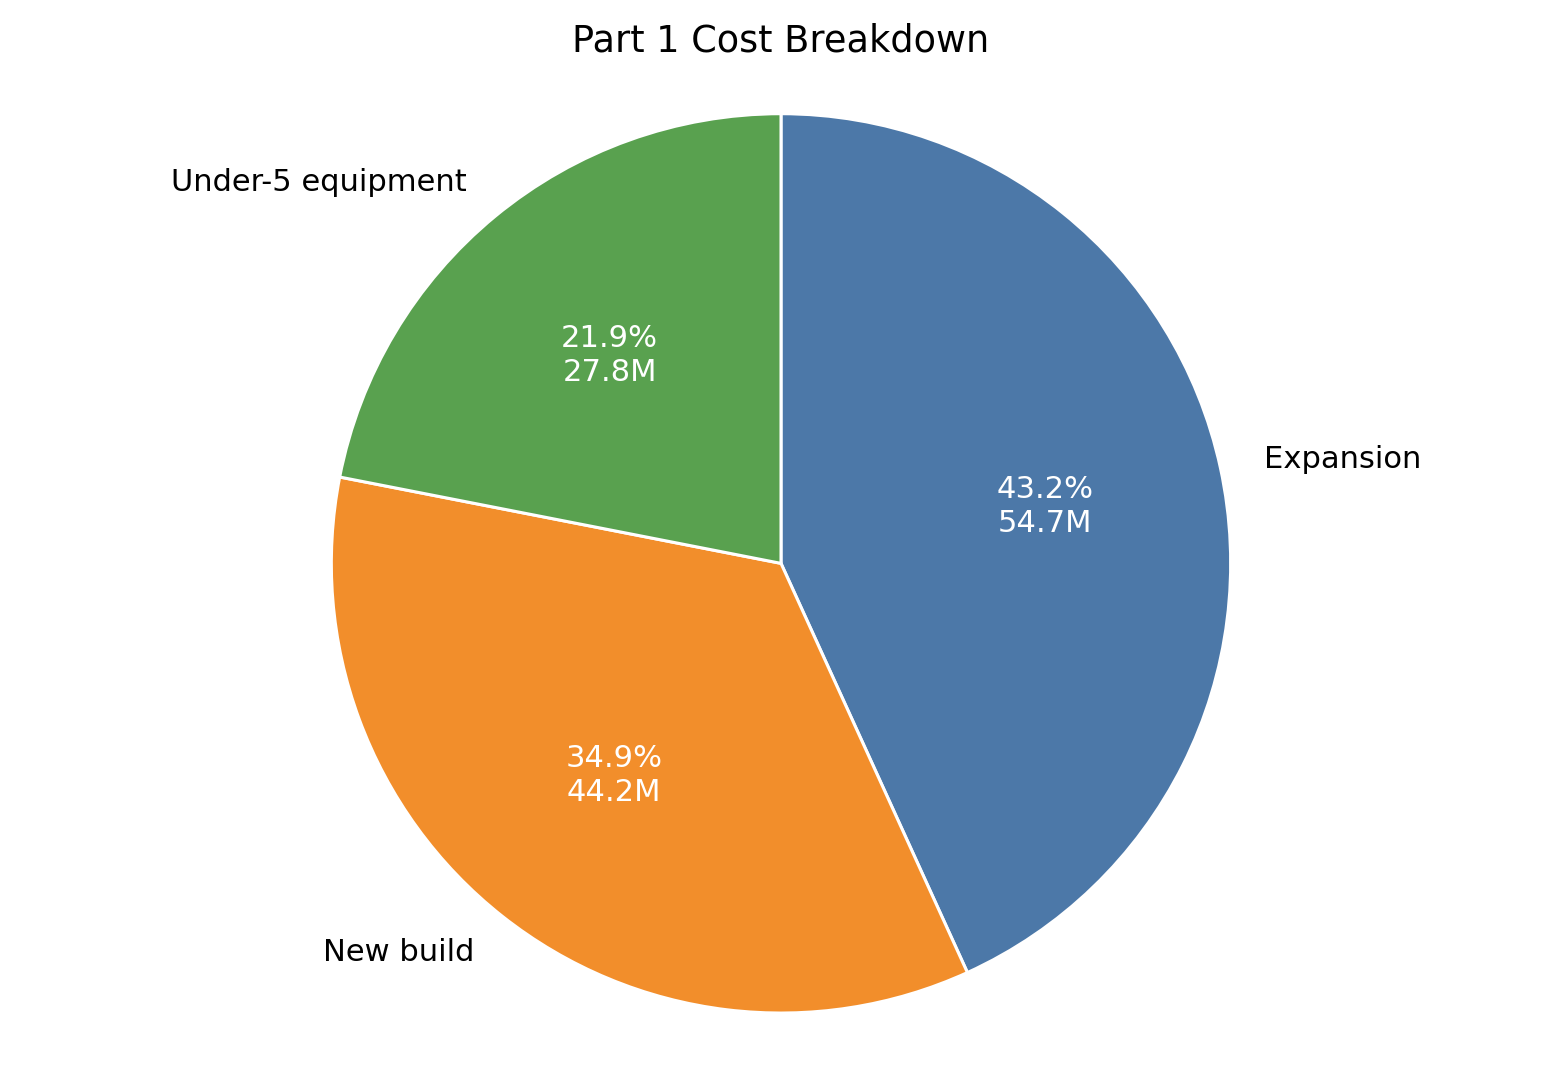
\includegraphics[width=0.78\textwidth]{ideal_cost_breakdown.png}
\caption{Part 1 cost breakdown from the exported ideal-model outputs}
\label{fig:ideal-cost-breakdown}
\end{figure}

\begin{resultbox}
\textbf{Benchmark takeaway.}
The corrected Part 1 model costs \(\$126.67\) million, combines \(206{,}364\) expansion slots with \(386\) new facilities, and pushes \(135\) existing facilities into the higher-cost expansion regime.
\end{resultbox}

\subsubsection{Interpretation}

The benchmark still relies heavily on incumbent expansion, but not exclusively. High-need zipcodes such as \(11219\), \(11230\), \(11223\), \(11368\), and \(11220\) still require several thousand added slots, so new construction remains necessary even under optimistic siting assumptions. The volume of under-\(5\) expansion also shows that the under-\(5\) requirement is the main system-wide driver.

The corrected threshold-cost logic matters. In the final solution, \(135\) facilities cross the \(x_f \ge n_f\) threshold and are priced entirely under the higher-cost rule, which tempers aggressive expansion and shifts part of the benchmark response toward new construction. Even the ideal model therefore implies a large capital program rather than a marginal adjustment.

\subsubsection{Limitations}

The strength of Part 1 is also its main limitation: it assumes a high degree of flexibility. In practice, new facilities cannot be opened arbitrarily within every zipcode, and existing facilities may face regulatory or physical barriers to expansion. The benchmark model also treats demand at the zipcode level and does not account for travel between neighborhoods. These limitations do not invalidate the model, but they do mean that its results should be interpreted as a planning benchmark rather than a deployable implementation plan. This motivates the realistic extension in Part 2.

\section{Part 2: Realistic childcare expansion model}

\subsection{Problem statement}

Part 2 keeps the same zipcode-level demand targets as Part 1, but changes the intervention mechanics. Existing facilities can expand only within a realistic \(20\%\) cap, new facilities must be placed on observed candidate sites, and new sites are screened against a within-zipcode spacing rule of \(0.06\) miles. The result is a substantially tighter decision space than in the benchmark model.

This is not simply a larger version of Part 1. It changes both the feasible actions and the economic trade-off. Once expansions become small, banded, and more expensive at higher levels, the model must rely much more heavily on new construction. The practical question becomes whether the city can still eliminate coded childcare deserts under these tighter siting and expansion rules, and if so, how expensive that plan becomes.

\subsection{Data and parameter construction}

\subsubsection{Realistic expansion parameters}

Implementation-wise, Part 2 plugs in immediately after the shared cleaning and zipcode-level parameter estimation work. The realistic parameter notebook reuses the cleaned facility and geography tables from the shared preprocessing stage and the zipcode-level demand table exported by the Part 1 parameter notebook; it does not depend on the optimal decision variables produced by the ideal model notebook. Starting from those shared inputs, Part 2 carries forward the upstream zero-child correction, screens candidate sites using coordinate-based distance rules, and assigns new realistic expansion parameters to existing facilities. For each active existing facility \(f\), we keep current total capacity \(n_f\) and the under-\(5\) proxy \(b_f\), then redefine the feasible expansion range to reflect the realistic policy recommendation that capacity cannot be increased by more than \(20\%\).

The realistic expansion cap is implemented through three blocks:
\[
\mathrm{cap1}_f = \left\lfloor 0.10\,n_f \right\rfloor,\qquad
\mathrm{cap2}_f = \left\lfloor 0.15\,n_f \right\rfloor - \left\lfloor 0.10\,n_f \right\rfloor,\qquad
\mathrm{cap3}_f = \left\lfloor 0.20\,n_f \right\rfloor - \left\lfloor 0.15\,n_f \right\rfloor
\]

These blocks correspond to the intervals \(0\%\) to \(10\%\), \(10\%\) to \(15\%\), and \(15\%\) to \(20\%\) of current capacity. Using cumulative floors preserves the intended total cap of \(\lfloor 0.20 n_f \rfloor\) at each facility. The current processed inputs imply a citywide realistic expansion capacity of \(61{,}197\) slots, which is still substantially smaller than the ideal benchmark's effective expansion room.

The corresponding block-specific cost coefficients follow the formulas used in the realistic parameter notebook:
\[
\mathrm{coef1}_f = \frac{20000 + 200\,n_f}{n_f},\qquad
\mathrm{coef2}_f = \frac{20000 + 400\,n_f}{n_f},\qquad
\mathrm{coef3}_f = \frac{20000 + 1000\,n_f}{n_f}
\]

\subsubsection{Candidate-site and distance parameters}

The realistic model uses the cleaned potential-locations dataset to define candidate sites for new construction. Each candidate site is combined with the same three build-size options from Part 1: small, medium, and large. The new-facility cost and capacity menu is therefore unchanged, but now every new opening must be placed at a specific observed site.

To operationalize the spacing requirement, we computed great-circle distances in miles between candidate sites and between candidate sites and existing facilities. A candidate site is blocked if it lies within \(0.06\) miles of an existing facility in the same zipcode. For candidate pairs in the same zipcode, any pair closer than \(0.06\) miles is added to a conflict table so that both sites cannot be selected simultaneously. Existing-existing pairs below the same threshold are tracked only diagnostically because existing facilities are fixed and cannot be removed.

\begin{table}[H]
\centering
\small
\begin{tabular}{lr}
\toprule
\textbf{Screening metric} & \textbf{Value} \\
\midrule
Candidate sites examined & 31,100 \\
Blocked candidate sites & 2,578 \\
Feasible candidate sites & 28,522 \\
Candidate-candidate conflict pairs & 11,455 \\
Candidate-existing conflict pairs & 4,730 \\
Existing-existing close pairs (diagnostic) & 7,644 \\
\bottomrule
\end{tabular}
\caption{Candidate-site screening summary for the realistic model}
\end{table}

\subsubsection{Build options and inherited assumptions}

The build menu from Part 1 is retained unchanged: small facilities contribute \((100, 50, \$65{,}000)\), medium facilities contribute \((200, 100, \$95{,}000)\), and large facilities contribute \((400, 200, \$115{,}000)\), where each tuple gives total capacity, under-\(5\) capacity, and fixed construction cost. As before, each newly created under-\(5\) slot carries an additional \(\$100\) equipment cost.

The demand side is inherited from the corrected Part 1 demand table. Part 2 therefore keeps the same high-demand classification rule, the same under-\(5\) requirement, and the same zipcode-level aggregation, while carrying forward the upstream rule that zipcodes with zero observed child population also have zero total-slot requirement.

\subsection{Optimization model}

\subsubsection{Modeling assumptions}

The realistic formulation uses the following assumptions:

\begin{enumerate}
    \item Demand requirements by zipcode follow the corrected Part 1 demand table, including zero total-slot requirement in zero-child zipcodes.
    \item Existing facilities remain fixed in place and may only expand within the realistic \(20\%\) cap.
    \item Expansion costs are modeled through three ordered blocks with increasing marginal cost.
    \item New facilities can only be opened at observed candidate sites.
    \item At most one facility size may be chosen at any candidate site.
    \item Candidate sites too close to existing facilities are blocked.
    \item Candidate sites that are too close to each other cannot both be selected.
    \item Existing-existing distance conflicts are recorded diagnostically but not enforced because the model does not relocate or close existing facilities.
    \item The same \texttt{children\_capacity} proxy is used for current under-\(5\) capacity at existing facilities.
\end{enumerate}

\subsubsection{Decision variables}

The realistic model extends the Part 1 decision structure by introducing candidate-site decisions. For each existing facility \(f\), we define:
\begin{itemize}
    \item \(x_{1f}, x_{2f}, x_{3f}\): expansion slots in the three realistic cost blocks;
    \item \(u_f\): under-\(5\) slots assigned within the expansion at facility \(f\).
\end{itemize}

\noindent
For each candidate site \(l\) and facility size \(s \in S\), we define:
\begin{itemize}
    \item \(y_{ls}\): a binary variable equal to \(1\) if a facility of size \(s\) is built at site \(l\);
    \item \(g_{ls}\): the number of under-\(5\) slots assigned within that selected new facility.
\end{itemize}

\subsubsection{Objective function}

The objective remains the minimization of total funding:
\[
\min \quad
\sum_{f \in F} \left(\mathrm{coef1}_f x_{1f} + \mathrm{coef2}_f x_{2f} + \mathrm{coef3}_f x_{3f}\right)
+
\sum_{l \in L} \sum_{s \in S} K_s y_{ls}
+
100\left(\sum_{f \in F} u_f + \sum_{l \in L} \sum_{s \in S} g_{ls}\right)
\]

As implemented in the repaired Part 2 pipeline, this objective uses additive block costs to preserve increasing marginal expansion costs in a tractable MILP. That is a modeling approximation to the assignment's more literal piecewise-total cost rule, which remains harder to solve at the same scale.

\subsubsection{Constraints}

The realistic model keeps the zipcode-level service constraints from Part 1 but adds several layers of feasibility restrictions.

First, each existing facility can expand only within the three block limits:
\[
x_{1f} \le \mathrm{cap1}_f,\qquad
x_{2f} \le \mathrm{cap2}_f,\qquad
x_{3f} \le \mathrm{cap3}_f
\qquad \forall f \in F
\]

Second, under-\(5\) slots created through expansion cannot exceed total added slots:
\[
u_f \le x_{1f} + x_{2f} + x_{3f}
\qquad \forall f \in F
\]

Third, each candidate site can host at most one facility size:
\[
\sum_{s \in S} y_{ls} \le 1
\qquad \forall l \in L
\]

Fourth, under-\(5\) assignments in selected new facilities cannot exceed the size-specific limit:
\[
g_{ls} \le U_s y_{ls}
\qquad \forall l \in L,\ \forall s \in S
\]

Fifth, blocked candidate sites are forced to remain unused, and any two candidate sites that form a conflict pair cannot both be selected:
\[
\sum_{s \in S} y_{ls} = 0
\qquad \forall l \in L_{\text{blocked}}
\]
\[
\sum_{s \in S} y_{l_1 s} + \sum_{s \in S} y_{l_2 s} \le 1
\qquad \forall (l_1,l_2) \in \mathcal{C}
\]

Finally, the zipcode-level total-capacity and under-\(5\)-capacity constraints are preserved from Part 1, except that new construction now enters through candidate sites rather than arbitrary zipcode-level build counts:
\[
\mathrm{existing\_total}_z
+
\sum_{f \in F(z)} (x_{1f}+x_{2f}+x_{3f})
+
\sum_{(l,s)\in L(z)} B_s y_{ls}
\ge \mathrm{req\_total}_z
\qquad \forall z \in Z
\]
\[
\mathrm{existing\_under5}_z
+
\sum_{f \in F(z)} u_f
+
\sum_{(l,s)\in L(z)} g_{ls}
\ge \mathrm{req\_under5}_z
\qquad \forall z \in Z
\]

\begin{resultbox}
\textbf{Implemented Part 2 model.}
Notebook 06 solves a citywide mixed-integer program with three integer expansion bands per existing facility, binary candidate-site choices for new facilities, zipcode-level total and under-\(5\) service constraints, and candidate-site conflict screening. The expansion objective is an additive increasing-cost approximation: it captures the intended rise in marginal cost, but it is not the literal piecewise-total formula from the assignment text.
\end{resultbox}

\subsection{Results and interpretation}

\subsubsection{Optimal solution summary}

The current realistic mixed-integer model is substantially larger than the ideal benchmark, with approximately \(201{,}980\) variables and \(155{,}819\) constraints. Gurobi solved it in about \(18.2\) seconds within the prescribed \(0.1\%\) optimality tolerance, with a final relative MIP gap of roughly \(0.090\%\). The resulting objective value is approximately \(\$183.96\) million.

Spending is dominated by new construction: \(\$9.38\) million for expansion, \(\$146.81\) million for new facilities, and \(\$27.77\) million for under-\(5\) equipment. The solution expands \(1{,}126\) existing facilities for \(25{,}108\) added slots and builds \(1{,}284\) new facilities for \(507{,}700\) slots. It also places no new facilities in zero-child zipcodes.

\begin{table}[H]
\centering
\small
\begin{tabular}{lr}
\toprule
\textbf{Quantity} & \textbf{Value} \\
\midrule
Total intervention cost (\$) & 183,963,207 \\
Expansion cost (\$) & 9,381,107 \\
New-build cost (\$) & 146,810,000 \\
Under-\(5\) equipment cost (\$) & 27,772,100 \\
Expanded facilities & 1,126 \\
Expanded total slots & 25,108 \\
Expanded under-\(5\) slots & 25,067 \\
New facilities built & 1,284 \\
New total slots & 507,700 \\
New under-\(5\) slots & 252,654 \\
\bottomrule
\end{tabular}
\caption{Summary of the optimal solution for the realistic model}
\end{table}

The solution meets the coded total-capacity and under-\(5\) requirements in all \(311\) zipcodes. New construction appears in \(180\) zipcodes and expansion in \(151\), and the size mix remains overwhelmingly large: \(1{,}261\) large facilities, \(10\) medium facilities, and \(13\) small facilities.

\subsubsection{Model verification}

We then ran explicit post-solve checks on zipcode feasibility, blocked-site exclusion, candidate-conflict enforcement, facility expansion limits, and zero-child zipcode handling.

\begin{resultbox}
\textbf{Post-solve checks all pass.}
All \(311\) zipcodes satisfy both service requirements; \(0\) blocked candidate sites are selected; \(0\) selected candidate pairs violate the candidate-candidate distance-conflict table; \(0\) facilities violate expansion or under-\(5\) assignment caps; and \(0\) zero-child zipcodes receive new facilities. These checks are exported directly from the realistic optimization stage.
\end{resultbox}

\begin{table}[H]
\centering
\small
\begin{tabular}{lrrr}
\toprule
\textbf{Metric} & \textbf{Part 1} & \textbf{Part 2} & \textbf{Change} \\
\midrule
Total cost (\$) & 126,668,941 & 183,963,207 & +57,294,267 \\
Expansion slots & 206,364 & 25,108 & -181,256 \\
New-build slots & 152,900 & 507,700 & +354,800 \\
New facilities & 386 & 1,284 & +898 \\
Under-\(5\) equipment cost (\$) & 27,772,100 & 27,772,100 & 0 \\
\bottomrule
\end{tabular}
\caption{Part 1 versus Part 2 intervention comparison}
\end{table}

The shift from benchmark flexibility to realistic siting restrictions is summarized graphically in \cref{fig:part-comparison-overview}.

\begin{figure}[H]
\centering
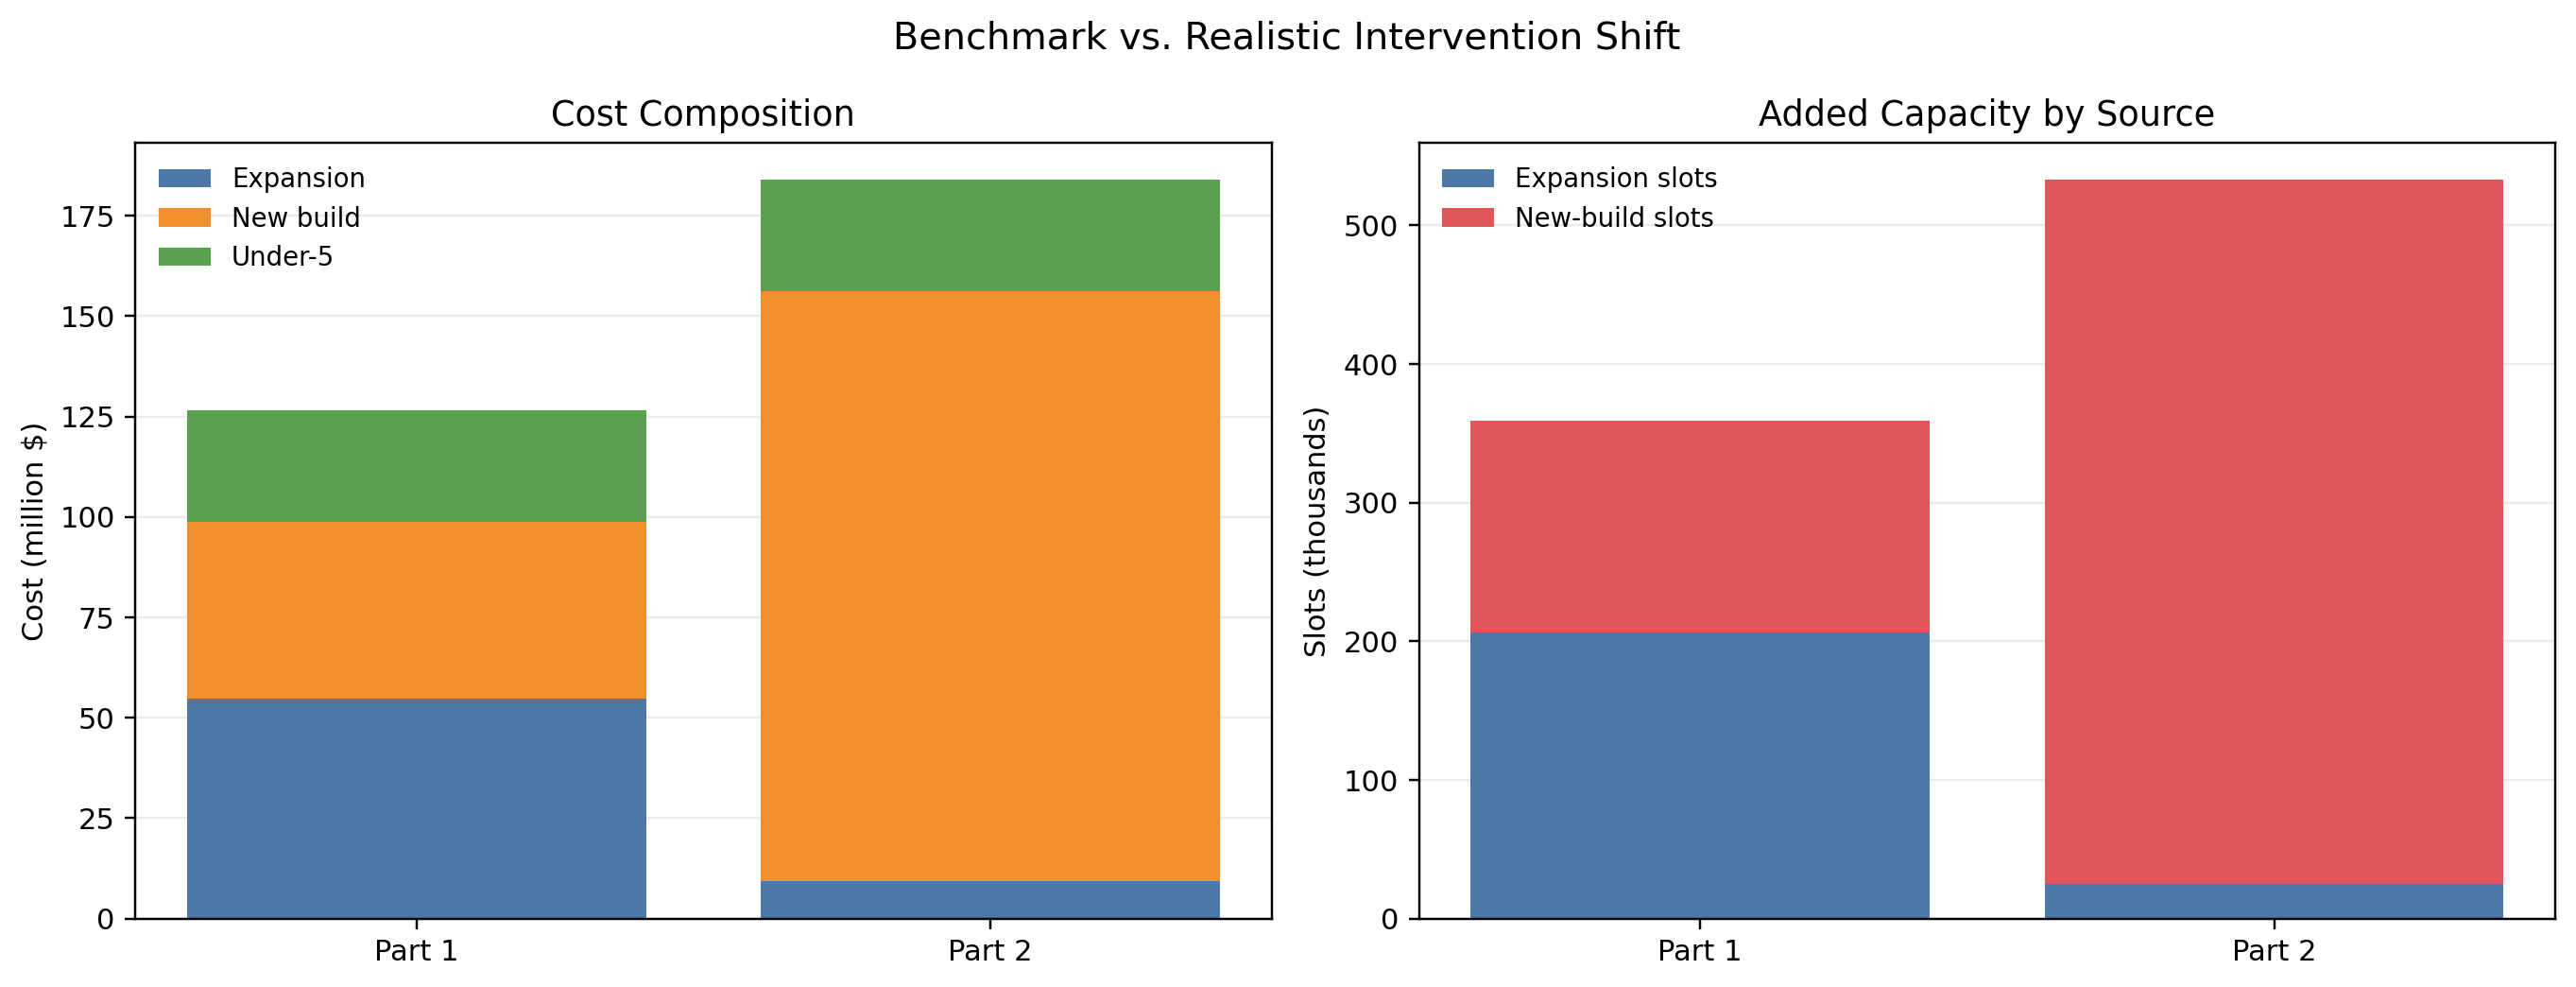
\includegraphics[width=\textwidth]{part_comparison_overview.png}
\caption{Cost and capacity composition shift from Part 1 to Part 2}
\label{fig:part-comparison-overview}
\end{figure}

\begin{resultbox}
\textbf{Main Part 2 shift.}
Relative to Part 1, realistic restrictions increase total cost by \(\$57.29\) million, reduce expansion by \(181{,}256\) slots, and require \(898\) additional new facilities. The policy burden shifts from expanding existing centers to financing many more large new builds.
\end{resultbox}

\subsubsection{Interpretation}

Relative to the ideal benchmark, the realistic model shifts decisively away from expansion and toward new construction. The \(20\%\) cap sharply limits incumbent growth, and the minimum-distance rule shrinks the feasible site menu. Even after carrying forward the corrected demand table and restored realistic expansion room, the city still needs \(1{,}284\) new facilities to deliver the same under-\(5\) coverage standard.

The under-\(5\) requirement remains the tightest system-wide constraint. All \(311\) zipcodes end with zero under-\(5\) slack, while only \(130\) have zero total-capacity slack, so the model creates visible total-capacity oversupply in order to deliver enough under-\(5\) slots through the available build menu. The largest interventions remain concentrated in \(11219\), \(11230\), \(11368\), \(11206\), \(11223\), and \(11204\), where new construction is clearly necessary rather than optional.

\begin{figure}[H]
\centering
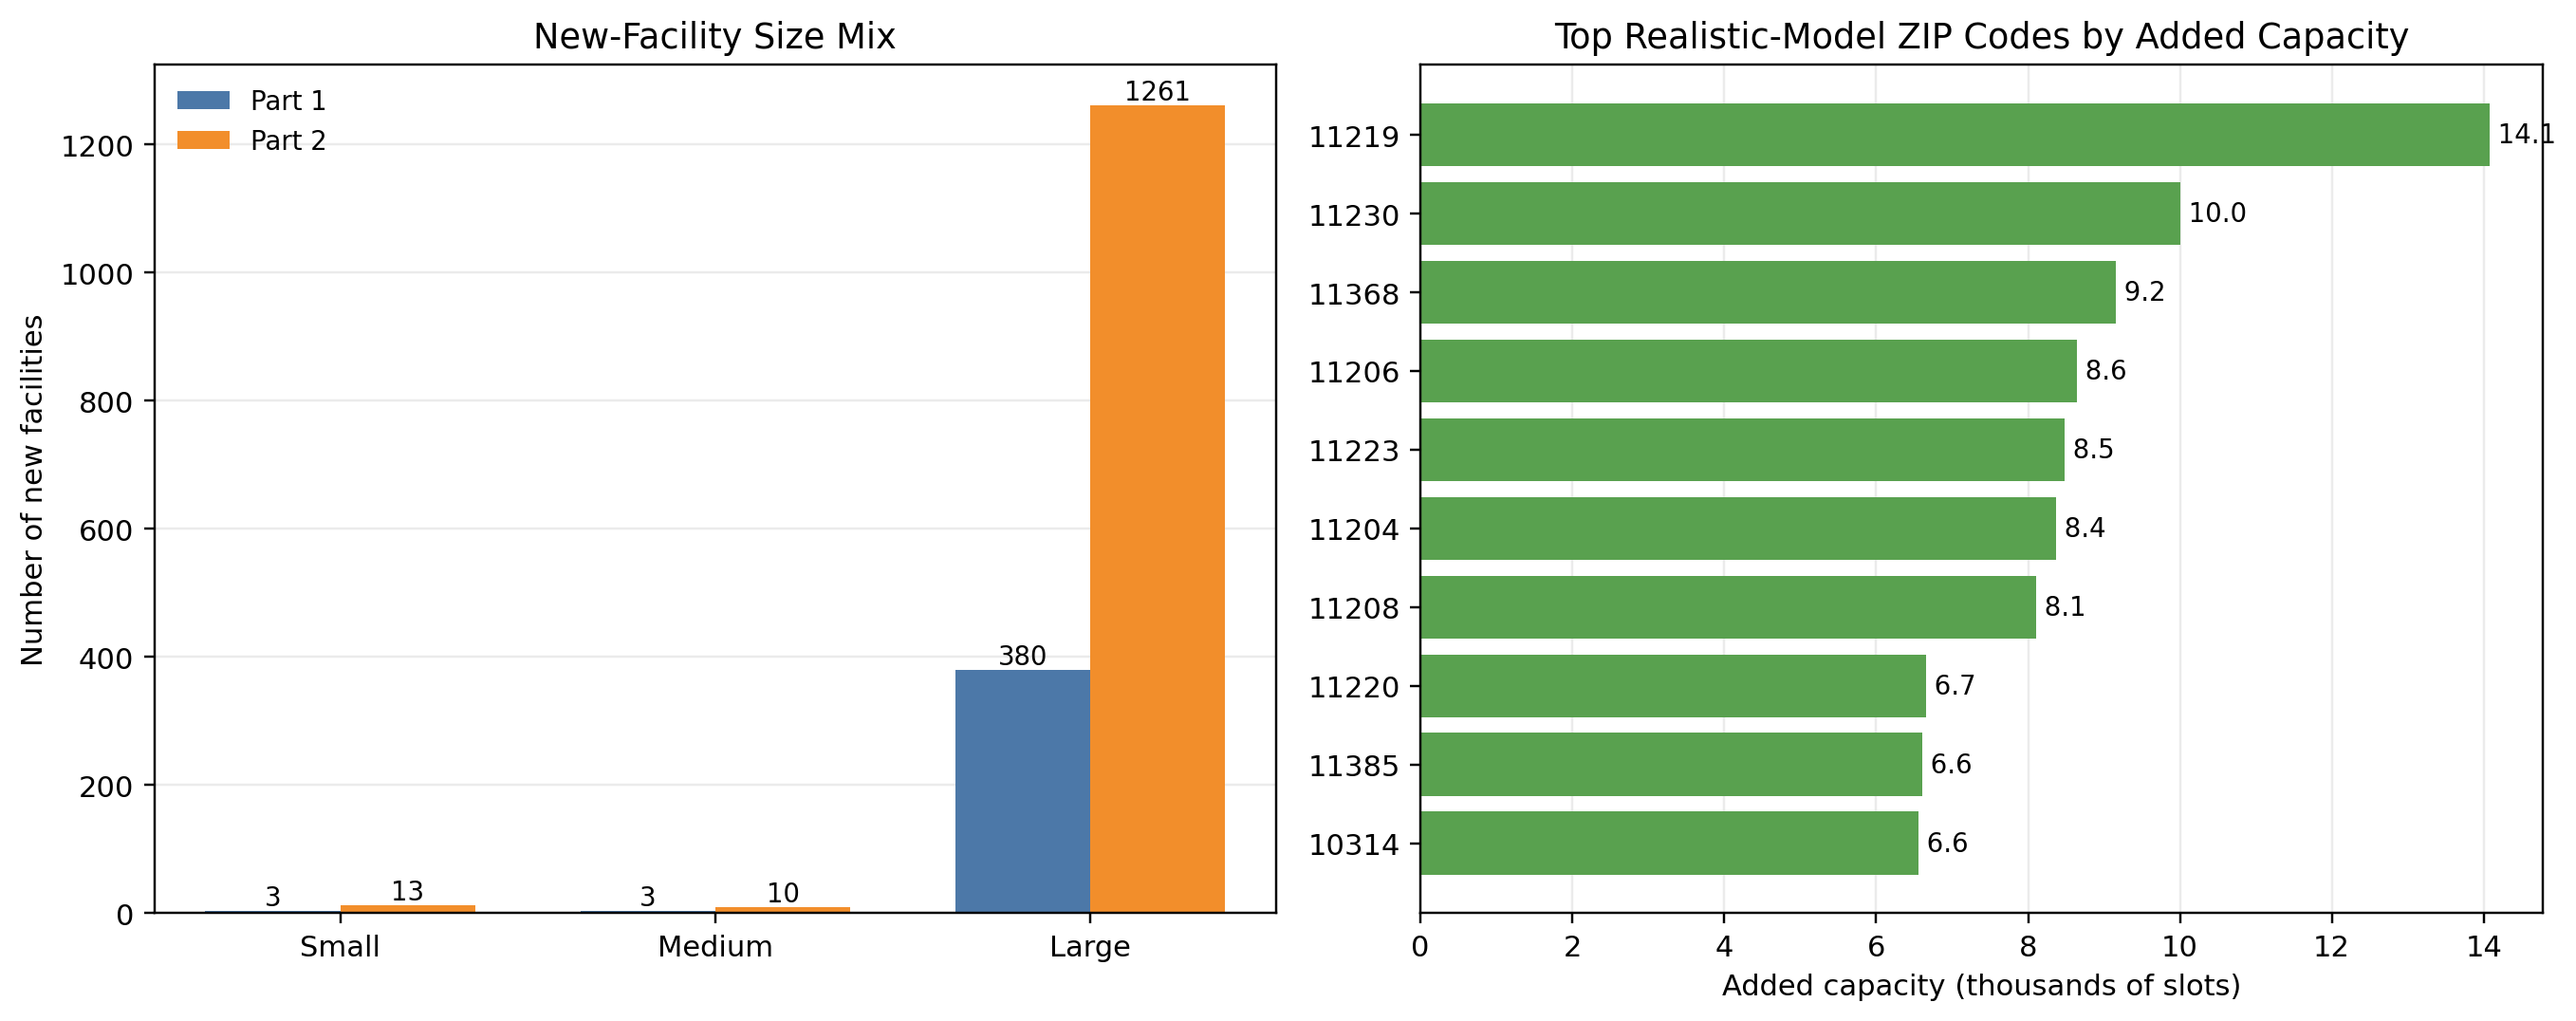
\includegraphics[width=\textwidth]{realistic_mix_and_zipcodes.png}
\caption{New-facility size mix and top added-capacity zipcodes in the realistic model}
\label{fig:realistic-mix-zips}
\end{figure}

\subsubsection{Limitations}

Although Part 2 is more operational than the benchmark model, it is still not a full deployment model. First, existing-existing distance conflicts are recorded diagnostically but are not enforced because existing facilities are fixed and cannot be closed or relocated within the current planning horizon. Second, distance screening is enforced only within zipcodes, so the model does not represent cross-zipcode competitive effects or household travel across boundaries. Third, \(169\) existing facilities still lack coordinates, which means that candidate-existing screening is only as accurate as the available geographic data. Finally, the current Part 2 pipeline still uses an additive block-cost approximation rather than the literal piecewise-total realistic cost rule, because the exact version is materially slower to solve at the current citywide scale.

\section*{Conclusions}
\addcontentsline{toc}{section}{Conclusions}

The two-stage analysis highlights both a cost increase and a mechanism change. Under benchmark flexibility, NYC can eliminate coded childcare deserts for approximately \(\$126.67\) million. Under realistic expansion and spacing rules, the objective rises to approximately \(\$183.96\) million, about \(45.2\%\) higher.

The main shift is away from incumbent expansion and toward large-scale new construction. Across both models, the under-\(5\) requirement remains the dominant planning driver, so practical policy discussion should focus not just on total slot creation, but on where under-\(5\) capacity can be delivered at scale.

\section*{Bibliography}
\addcontentsline{toc}{section}{Bibliography}

\begin{thebibliography}{9}
\bibitem{assignment}
IEOR E4004. \emph{Project I: Eliminating Child Care Deserts in New York City through Optimization}. Columbia University, Spring 2026.

\bibitem{factsheet}
IEOR E4004. \emph{Project I: Eliminating Child Care Deserts in New York City through Optimization --- Fact Sheet}. Columbia University, Spring 2026.

\bibitem{americanprogress}
Center for American Progress. \emph{Child Care Deserts in the United States}. Available at \url{https://www.americanprogress.org/series/child-care-deserts/}.
\end{thebibliography}

% ===========================
% APPENDIX PLACEHOLDER
% ===========================
\appendix

\section*{Appendix}
\addcontentsline{toc}{section}{Appendix}

Detailed solver logs, zipcode-level outputs, facility-level outputs, and exported tables used to prepare the report are available in the project repository.
The report figures in this document are generated from the dedicated Notebook 07 visualization workflow and exported to \texttt{report/figures/}.

% ===========================
\end{document}
